% CHAPTER 4
\chapter{Implementation}

\section{Hardware and Software Requirements}

The development, training, and deployment of SARAS was executed across a hybrid computational pipeline comprising a deep learning workstation, a high-fidelity robotic simulation cluster, and physical embedded UAV hardware:

\subsection{Workstation Training and Simulation Environment}
\begin{itemize}
    \item \textbf{Processor (CPU):} Intel Core i7-12700H (14 cores, 20 threads, up to 4.7 GHz base/boost clock).
    \item \textbf{Graphics Accelerator (GPU):} NVIDIA GeForce RTX 3070 Ti Laptop GPU (8 GB GDDR6 VRAM, 5,888 CUDA cores, 184 Tensor cores).
    \item \textbf{System Memory (RAM):} 32 GB dual-channel DDR5 @ 4800 MHz.
    \item \textbf{Operating System:} Ubuntu 22.04 LTS (Jammy Jellyfish) 64-bit kernel with dual-boot Windows 11 environment.
    \item \textbf{CUDA / cuDNN Stack:} NVIDIA CUDA Toolkit v11.8 with cuDNN v8.7.0 acceleration libraries.
    \item \textbf{Python Runtime:} Python v3.10.12 virtual environment.
\end{itemize}

\subsection{Physical UAV and Embedded Edge Hardware}
\begin{itemize}
    \item \textbf{Airframe Platform:} Holybro S500 quadcopter frame ($500\text{ mm}$ motor-to-motor wheelbase) constructed with carbon-fiber reinforced arms.
    \item \textbf{Flight Controller Unit (FCU):} Pixhawk 4 Autopilot with STM32F765 32-bit ARM Cortex-M7 processor running PX4 Autopilot firmware v1.14.
    \item \textbf{Embedded Companion Computer:} Raspberry Pi 4 Model B (Broadcom BCM2711 quad-core ARM Cortex-A72 @ 1.5 GHz, 4 GB LPDDR4 RAM, running Raspberry Pi OS 64-bit Debian bullseye).
    \item \textbf{Perception Sensor:} Raspberry Pi Camera Module v2 equipped with an 8-megapixel Sony IMX219 sensor configured for $1920 \times 1080$ capture at 30 FPS.
    \item \textbf{Power Distribution and Propulsion:} 4S 5000 mAh 35C Lithium-Polymer (LiPo) battery supplying 14.8 V nominal voltage, paired with 2216 880 KV brushless DC motors and 1045 propellers.
    \item \textbf{Telemetry Communications:} Holybro 500 mW 433 MHz Sik radio transceivers for long-range MAVLink telemetry, paired with an onboard dual-band 802.11ac Wi-Fi module for inter-agent mesh communication.
\end{itemize}

\section{Tools and Frameworks}

Table \ref{tab:tools} enumerates the primary software libraries, toolkits, and platforms utilized in the SARAS implementation, summarizing the dedicated functional role of each component:

\begin{table}[htbp]
\centering
\caption{Software toolkits, frameworks, and libraries utilized in the SARAS platform}
\label{tab:tools}
\vspace{0.2cm}
\resizebox{0.95\columnwidth}{!}{
\begin{tabular}{|l|l|l|}
\hline
\textbf{Tool / Library} & \textbf{Version} & \textbf{Functional Purpose in Project} \\
\hline
PyTorch & 2.0.1 & Deep learning framework utilized for model definition, tensor ops, and gradient backpropagation. \\
\hline
Ultralytics YOLOv8 & 8.0.196 & Computer vision package providing anchor-free decoupled head architectures and Mosaic augmentation. \\
\hline
ONNX Runtime & 1.15.1 & High-performance inference engine used to execute INT8 quantized models directly on ARM companion CPUs. \\
\hline
OpenCV & 4.8.0 & Computer vision toolkit used for video stream decoding, affine transforms, and visual bounding box overlays. \\
\hline
ROS 2 & Humble & Distributed robotic middleware used for inter-node message passing, state estimation, and sensor transforms. \\
\hline
Gazebo Harmonic & 7.5.0 & Multi-robot physics simulator providing accurate aerodynamic, gravity, and obstacle rendering for swarms. \\
\hline
PX4 Autopilot & 1.14.0 & Open-source flight stack managing low-level PID attitude control, EKF2 sensor fusion, and fail-safe modes. \\
\hline
MAVSDK-Python & 1.4.9 & Asynchronous client library interfacing companion computer scripts to the Pixhawk via MAVLink. \\
\hline
Next.js / Tailwind & 14.1.0 & Modern React web framework utilized to engineer the responsive, real-time Ground Control Dashboard. \\
\hline
Leaflet.js & 1.9.4 & Open-source mapping library used to render interactive GIS satellite tiles, sector bounds, and drone breadcrumbs. \\
\hline
FAISS / LangChain & 0.1.4 & Vector similarity index and multi-agent framework powering the RAG disaster triage decision support. \\
\hline
\end{tabular}
}
\end{table}

\section{Dataset Partitioning}

The training, validation, and benchmarking of the onboard perception system was structured around the official benchmark split of the VisDrone dataset \cite{16}:
\begin{itemize}
    \item \textbf{Training Partition:} Comprises 6,471 images (63.4\% of total samples), containing 343,204 labeled bounding box instances across variable environmental conditions.
    \item \textbf{Validation Partition:} Comprises 548 images (5.4\% of total samples), containing 38,912 target instances, utilized for periodic loss evaluation and early-stopping regularization during training.
    \item \textbf{Testing Partition:} Comprises 3,190 images (31.2\% of total samples), reserved strictly for post-training evaluation, generalization testing, and comparative benchmarking against published baseline models.
\end{itemize}
The partition employs a geographical and scene-stratified separation policy: flight sequences captured in identical disaster simulation runs or urban zones are strictly sequestered into disjoint partitions to prevent data leakage across frames.

\section{Hyperparameter Settings}

Table \ref{tab:hyperparameters} outlines the complete hyperparameter configuration utilized during the training of the SARAS edge vision detector:

\begin{table}[htbp]
\centering
\caption{Hyperparameter settings for edge object detector training}
\label{tab:hyperparameters}
\vspace{0.2cm}
\begin{tabular}{|l|l|}
\hline
\textbf{Hyperparameter} & \textbf{Configured Value} \\
\hline
Base Input Resolution & $640 \times 640$ pixels \\
\hline
Total Epochs & 100 \\
\hline
Batch Size & 16 \\
\hline
Optimization Algorithm & AdamW \\
\hline
Initial Learning Rate ($\eta_0$) & $1.0 \times 10^{-2}$ \\
\hline
Minimum Learning Rate ($\eta_{\text{min}}$) & $1.0 \times 10^{-4}$ \\
\hline
Learning Rate Schedule & Cosine Annealing with 3 Warmup Epochs \\
\hline
Momentum Parameters & $\beta_1 = 0.937, \beta_2 = 0.999$ \\
\hline
Weight Decay ($\omega$) & 0.0005 \\
\hline
Box Loss Gain ($\lambda_{\text{box}}$) & 7.5 \\
\hline
DFL Loss Gain ($\lambda_{\text{dfl}}$) & 1.5 \\
\hline
Classification Loss Gain ($\lambda_{\text{cls}}$) & 0.5 \\
\hline
Non-Maximum Suppression (NMS) IoU Threshold & 0.70 \\
\hline
Confidence Scoring Threshold & 0.25 \\
\hline
\end{tabular}
\end{table}

\section{Model Training Procedure}

The end-to-end model training procedure follows a disciplined execution sequence:
\begin{enumerate}
    \item \textbf{Data Pipeline Ingestion:} Images and label tensors are asynchronously loaded into pinned GPU memory using PyTorch `DataLoader` workers with persistent memory caching.
    \item \textbf{Warmup and Frozen Stage (Epochs 1--10):} For the first 3 epochs, the learning rate increases linearly from $1.0 \times 10^{-4}$ to $1.0 \times 10^{-2}$. The CSPDarknet backbone weights remain frozen during the initial 10 epochs, allowing decoupled detection heads to adapt their projection weights.
    \item \textbf{Full Backpropagation Stage (Epochs 11--100):} All model weights are unlocked. Gradients are computed using mixed-precision FP16 operations via NVIDIA Automatic Mixed Precision (AMP), reducing VRAM occupancy while maintaining numerical stability.
    \item \textbf{Validation Checkpoints and Early Stopping:} At the termination of each epoch, $\text{mAP@0.5}$ is evaluated on the validation partition. If validation mAP fails to improve for 15 consecutive epochs, training terminates automatically.
    \item \textbf{Post-Training Quantization (PTQ) Compilation:} The converged PyTorch checkpoint (`best.pt`) is exported to standard ONNX intermediate representation, followed by 8-bit integer symmetric quantization using calibration datasets.
\end{enumerate}
The complete training run converged at epoch 84 in \textbf{3 hours, 42 minutes, and 18 seconds} on the RTX 3070 Ti workstation.

\section{Deployment and Ground Control Interface}

The operational deployment of the SARAS platform spans onboard companion software and a browser-based ground command center:

\begin{figure}[htbp]
\centering
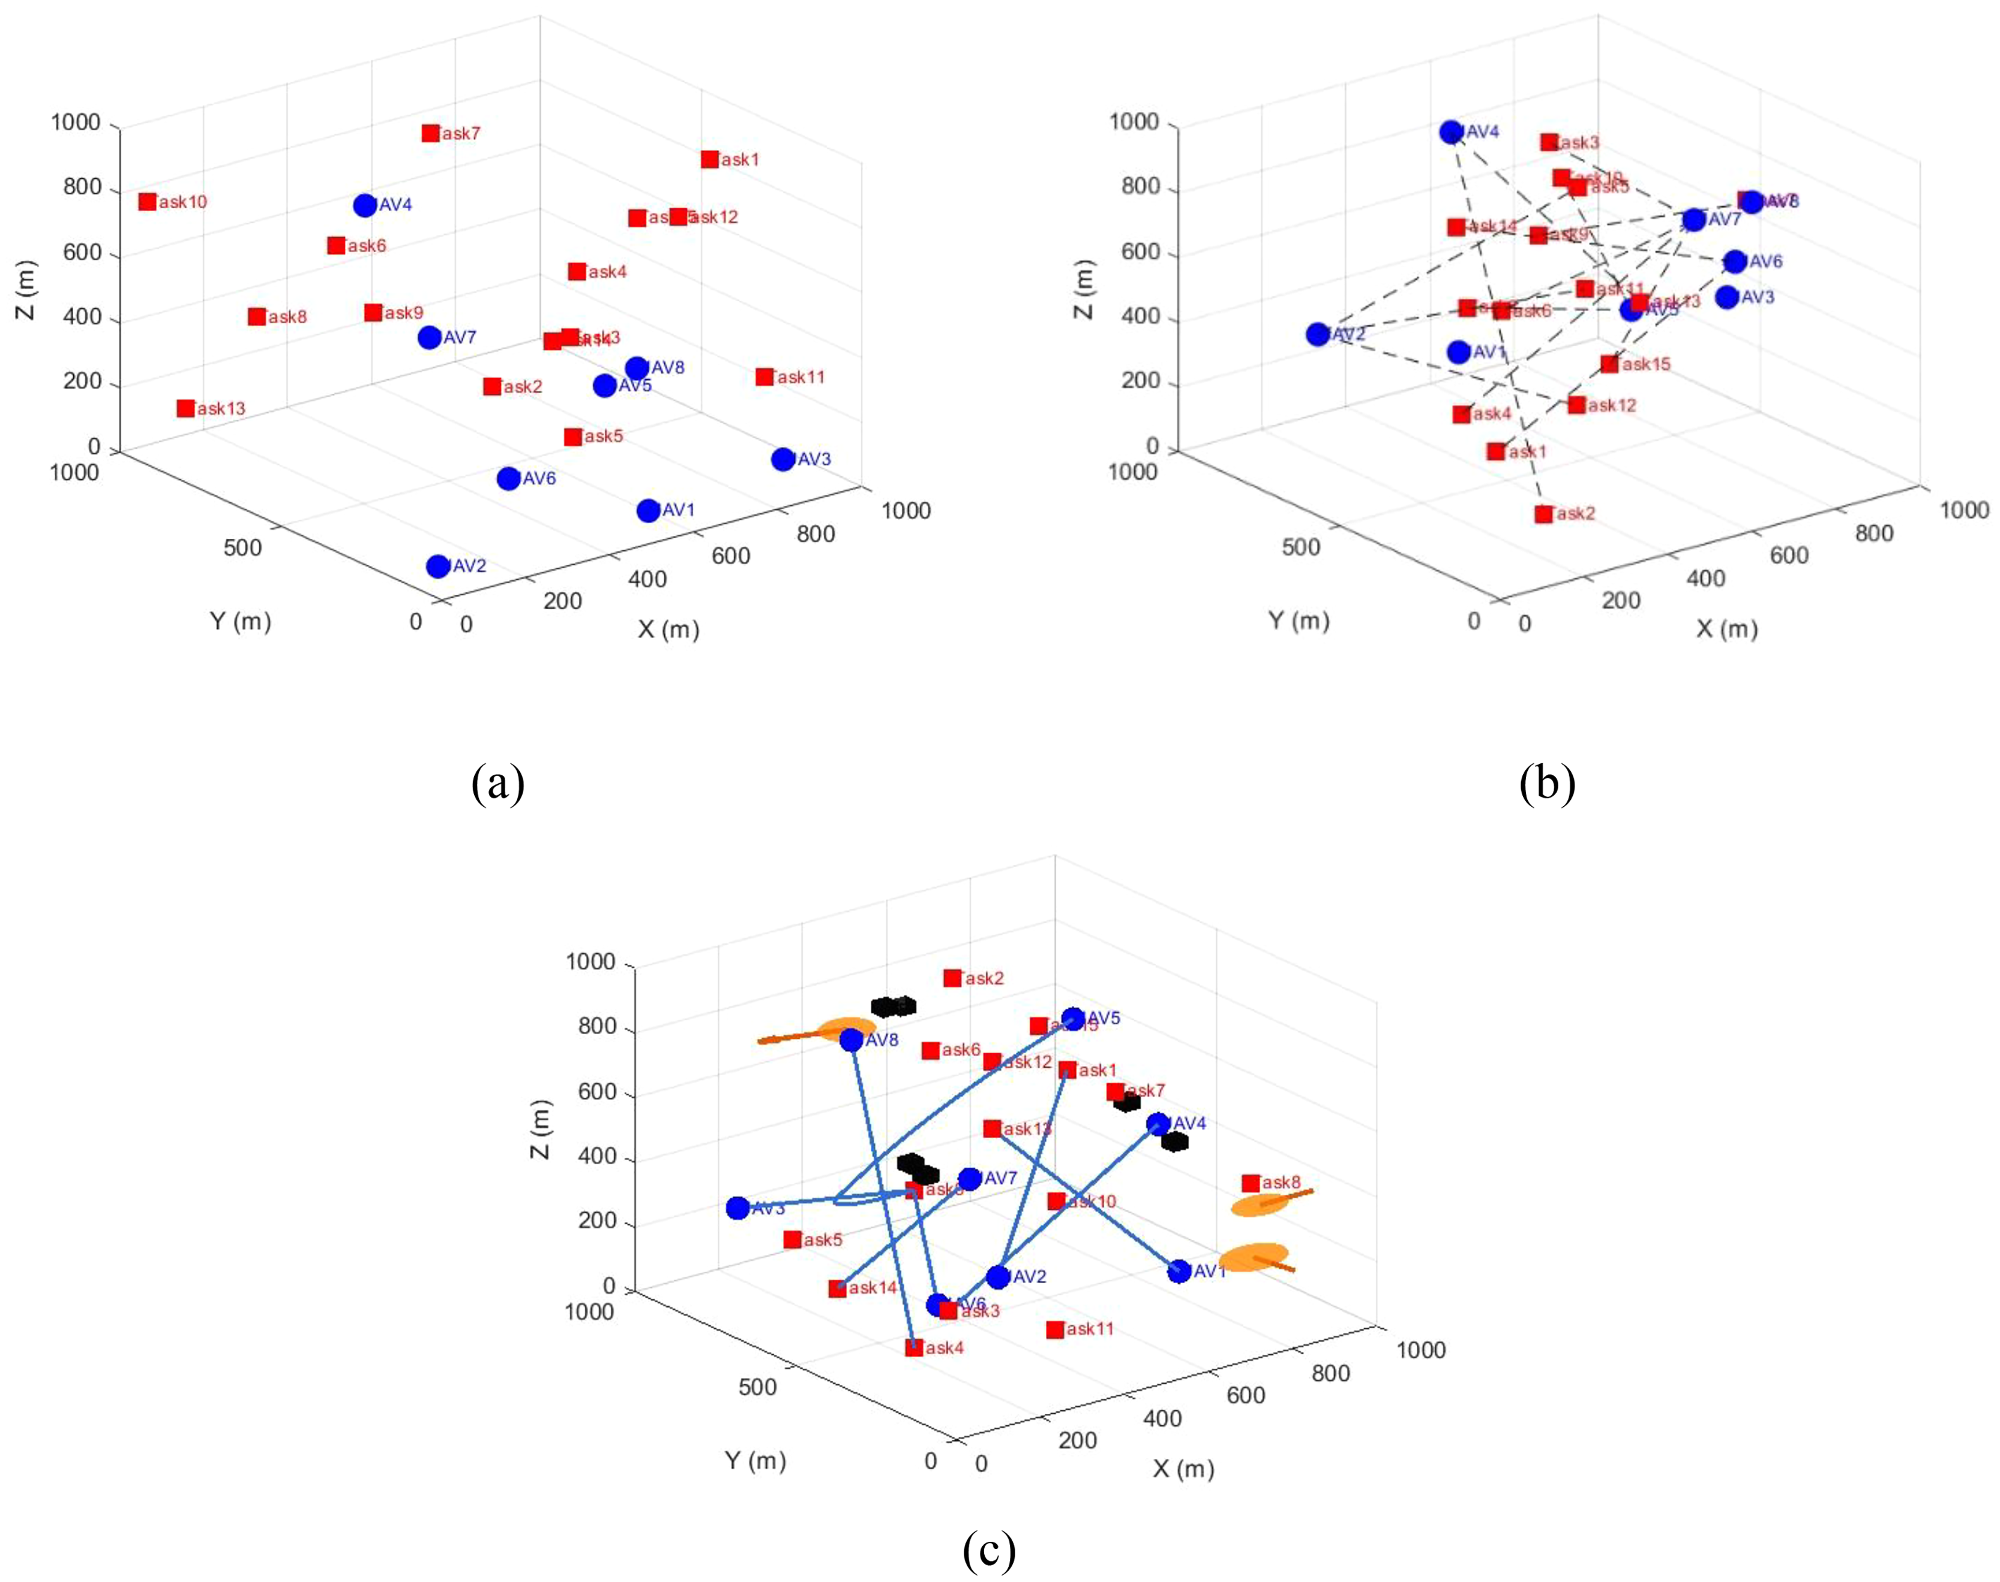
\includegraphics[width=0.88\textwidth]{assets/saras_simulation_setup.png}
\caption{Multi-UAV Gazebo simulation setup and physical quadcopter integration testbed}
\label{fig:sim_setup}
\end{figure}

\subsection{Onboard Edge Deployment}
The quantized INT8 ONNX model runs on the companion Raspberry Pi 4 inside a multithreaded Python daemon. Thread 1 captures frames from the Sony IMX219 sensor via Video4Linux2 (V4L2); Thread 2 executes ONNX Runtime inference using ARM NEON SIMD vector extensions; Thread 3 queries the Pixhawk FCU via MAVSDK to fetch current GPS coordinates, altitude Above Ground Level (AGL), and camera gimbal pitch, computing georeferenced survivor coordinates via flat-earth projection matrices.

\subsection{Interactive Ground Control Dashboard}
The ground station software is built using Next.js 14, providing incident commanders with situational awareness:
\begin{itemize}
    \item \textbf{Geospatial Sector Canvas:} Renders Leaflet GIS satellite maps displaying active search boundaries, dynamically color-coded by operational status: \textit{Unassigned} (Amber), \textit{In-Progress} (Blue), and \textit{Completed} (Green).
    \item \textbf{Live Telemetry Teleconference:} Streams real-time flight parameters (battery percentage, groundspeed, altitude, link quality) across an asynchronous WebSocket server.
    \item \textbf{Casualty Triage Console and RAG Terminal:} When victim detections are logged, casualty markers are plotted on the map. The built-in agentic RAG module accepts natural language commander queries (e.g., \textit{``What is the evacuation protocol for an unconscious casualty in flood terrain?''}) and returns citation-grounded emergency steps in under 1.2 seconds.
\end{itemize}
